% Convert with command:
% convert -density 300 pic.pdf -quality 90 pic.png
\documentclass[crop,tikz,border=0pt]{standalone}
\usetikzlibrary{arrows.meta, fit}
\begin{document}

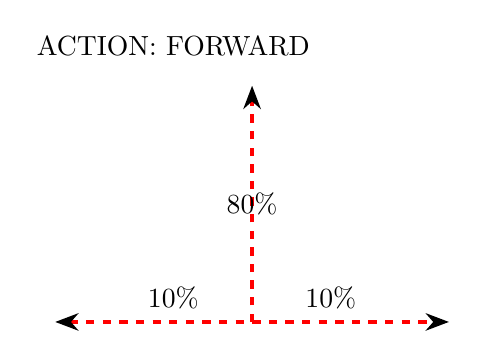
\begin{tikzpicture}

\draw[] (1.5, 3.5) node[] {ACTION: FORWARD};

\begin{scope}[>={Stealth[black]},
              every edge/.style={draw=red,very thick}]
    \path [<->,dashed] (0, 0) edge node {} (5, 0);
    \path [->,dashed] (2.5, 0) edge node {80\%} (2.5, 3);
    \draw[] (1.5, 0.3) node {10\%};
    \draw[] (3.5, 0.3) node {10\%};
\end{scope}
\end{tikzpicture}

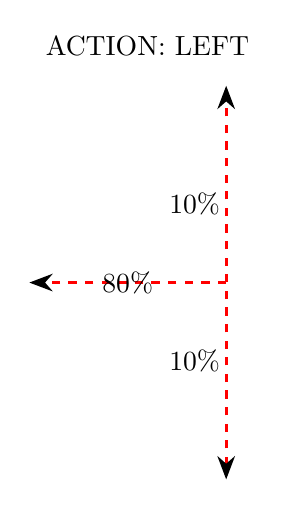
\begin{tikzpicture}
\draw[] (1.5, 3.5) node[] {ACTION: LEFT};
\begin{scope}[>={Stealth[black]},
              every edge/.style={draw=red,very thick}]
    \path [<->,dashed] (2.5, -2) edge node {} (2.5, 3);
    \path [->,dashed] (2.5, 0.5) edge node {80\%} (0, 0.5);
    \draw[] (2.1, -0.5) node {10\%};
    \draw[] (2.1, 1.5) node {10\%};
\end{scope}
\end{tikzpicture}

\begin{tikzpicture}
\draw[] (1.5, 3.5) node[] {ACTION: RIGHT};
\begin{scope}[>={Stealth[black]},
              every edge/.style={draw=red,very thick}]
    \path [<->,dashed] (2.5, -2) edge node {} (2.5, 3);
    \path [->,dashed] (2.5, 0.5) edge node {80\%} (5, 0.5);
    \draw[] (2.9, -0.5) node {10\%};
    \draw[] (2.9, 1.5) node {10\%};
\end{scope}
\end{tikzpicture}

\end{document}
